\newpage

\pagestyle{empty}
\xiaoer \textbf{保证和声明}
\vspace{0.7cm}

\xiaosi \textbf{商标信息}\\
%
\includegraphics[height=2cm]{logo}
%\epsfig{figure=logo,height=2cm}
%\begin{figure}[H]
%    
\includegraphics[height=2cm]{logo}
%\end{figure}
\hspace{8cm}\song{11\qquad\qquad 是合肥量精密仪器有限公司的注册商标。}
\hspace{-9.6cm}
\includegraphics[height=2cm]{logo}

\vspace{0.4cm}
\xiaosi\textbf{软件版本}

\song 软件升级可能会更改或增加产品功能, 请联系合肥量子精密仪器有限公司升级软件, 必要时我司会主动与您联系。

\vspace{0.4cm}
\xiaosi\textbf{声明}
\song
\begin{itemize}
 \item 本公司产品受中国及其他国家和地区的专利( 包括已取得和正在申请的专利)保护。
 \item 本公司拥有改变产品规格及价格的权利。
 \item 本手册提供的信息取代以往出版的任何资料。
 \item 未经我司事先书面许可, 不得影印、 复制或改变本手册的任何部分。
 \item 用户一旦使用本产品, 即视为对本声明的全部内容认可和接受。
\end{itemize}

\vspace{0.4cm}
\xiaosi\textbf{产品认证}
\vspace{3cm}

\xiaosi\textbf{联系我们}

\noindent\song
如果您在使用此产品或本手册的过程中有任何问题或需求,可与我司联系:\\
秦熙: 合肥量子精密仪器有限公司, 首席技术官\\
电子邮箱: sale@qpdtek.com\\
电话: +86 13816630636

\newpage
\xiaoer \textbf{安全要求}
\vspace{1.1cm}

\noindent\sanhao\textbf{一般安全概要}
\vspace{0.7cm}
\song

用户需了解以下安全预防措施, 以避免受伤, 并防止损坏本产品或与本产品连接的任何设备。 为避免可能的危险, 请务必按照规定使用本产品。

\vspace{0.6cm}
\noindent{\color{red}\textbf{使用正确的电源线}}

只允许使用我司所提供随机箱附件中的电源线。

\vspace{0.6cm}
\noindent{\color{red}\textbf{查看所有额定值}}

为避免过大电流的冲击, 造成人员受伤或仪器损坏, 请在使用产品前仔细阅读本手册以了解产品额定值的详细信息。

\vspace{0.6cm}
\noindent{\color{red}\textbf{确保供电电源正确}}

确保产品供电电源正确, 以免过高电压到达本产品对操作人员造成伤害, 并
损坏产品。

\vspace{0.6cm}
\noindent{\color{red}\textbf{请勿开盖操作}}

请勿在仪器机箱打开时运行本产品。

\vspace{0.6cm}
\noindent{\color{red}\textbf{避免电路外露}}

若机箱内电路板元件有外露, 请勿触碰上面的元件并立即与我司联系。

\vspace{0.6cm}
\noindent{\color{red}\textbf{怀疑产品出故障时, 请勿进行操作}}

如果您怀疑本产品出现故障, 请联络我司授权的维修人员进行检测。 任何由未经我司允许的维护、 调整或零件更换而造成损失, 我司不承担任何责任。

\vspace{0.6cm}
\noindent{\color{red}\textbf{保持良好的散热条件}}

在使用本产品的过程中切勿堵住通风口, 以免内部电路板过热而损坏仪器。

\vspace{0.6cm}
\noindent{\color{red}\textbf{请勿在潮湿环境下操作仪器}}

为避免仪器内部电路出现短路等危险情况, 请勿在潮湿环境下操作仪器。


\vspace{0.6cm}
\noindent{\color{red}\textbf{请勿靠近易燃易爆物品}}

为避免人身伤害或仪器损坏, 请勿让本产品靠近易燃易爆物品。

\vspace{0.6cm}
\noindent{\color{red}\textbf{注意搬运安全}}

为避免对仪器面板上的按键、 接口、 指示灯等部件造成损坏, 请注意搬运安全。

\newpage
%\vspace{0.6cm}
\noindent{\color{red}\textbf{远离高温环境}}

严禁将仪器至于高温环境中, 以免发生危险。

\vspace{0.5cm}
\noindent{\color{red}\textbf{严禁不具备操作能力的人使用本产品}}

严禁不具备操作能力的人使用本产品( 如老人、 儿童) , 以免造成人身伤害或仪器损坏。

\vspace{0.5cm}
\noindent{\color{red}\textbf{保养与清洁}}

请经常对仪器进行清洁, 方法如下: 先断开电源, 再用干抹布轻轻擦拭仪器机箱外部。

\newpage
%\pagestyle{plain}
%\setcounter{page}{1}
\noindent\huge \textbf{ASG-GT50-C} \xiaoer\textbf{任意序列发生器简介}
\vspace{0.6cm}

\normalsize ASG-GT50-C\song 系列是我司研发的高性能方波/延时发生器,又称任意序列发生器。该任意序列发生器不仅具有8个功能完全相同的方波输出通道,且集成了高速的计数读出功能。如下面的方波时序图所示,该仪器可以连续输出最短5 ns,最长达2.6 s宽度的方波,且无死时间,同时每个方波上升沿和下降沿的时间分辨率可达50 ps。
\begin{figure}[ht]
\centering
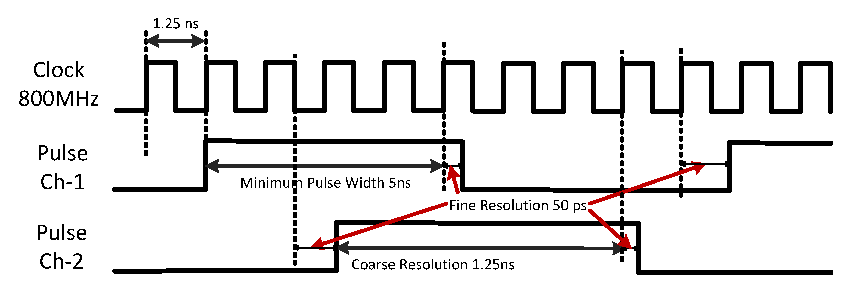
\includegraphics[width=14cm]{fig1}
\caption{方波时序图}\label{fig:fig1}
\end{figure}
\vspace{0.9cm}

\noindent\sanhao\textbf{产品主要特征}
\vspace{0.6cm}
\song
\begin{itemize}
 \item 50 ps时间分辨率的方波输出。
 \item 8个通道独立自定义方波输出。
 \item 单脉冲动态范围为5 ns至2.6 s,且无死时间。
 \item 高长期稳定度。
 \item 集成了高速计数读出功能。
 \item 方波序列的存储内存可以达到4 GB。
 \item 采用USB接口通信。
 \item 配备方波序列编辑软件。
\end{itemize}

\vspace{0.6cm}
\noindent\sanhao\textbf{产品技术规格参数}
\vspace{0.6cm}

\noindent\xiaosi\textbf{外观特征:}
\vspace{0.4cm}
\song
\begin{itemize}
 \item 机身材质: 铝合金外壳
 \item 机身颜色: 银灰色
 \item 产品尺寸: 207*122*65 mm
\end{itemize}

\vspace{0.4cm}
\noindent\xiaosi\textbf{电气特性:}
\vspace{0.4cm}
\song
\begin{itemize}
 \item 工作电压: DC 12 V
 \item 待机电流: 约 0.85 A
 \item 工作电流: ≤1.2 A
 \item 最大功率: 约 12 W
\end{itemize}

\vspace{0.4cm}
\noindent\xiaosi\textbf{技术参数:}
\vspace{0.4cm}
\song
\begin{itemize}
 \item  时间分辨率: 50 ps
 \item 最小脉冲宽度: 5 ns
 \item 最大脉冲宽度: 2.6 s
 \item 最大方波输出通道数: 8
 \item  方波序列存储内存: 4 GB
 \item  单通道最多输出方波个数: $4\times 10^8$个
 \item  耦合方式: DC 50 ohm
 \item  输出低电平: 0 V
 \item  输出高电平: 3.3 V
 \item  输入低电平: -5.2 V 至 +0.4 V
 \item  输入高电平: +0.6 V 至 +3.5 V
 \item  最大计数率: 50 MHz
 \item  单个计数使能信号脉冲宽度范围: 5 ns 至 5000 s
\end{itemize}

\vspace{1cm}
\noindent\sanhao\textbf{产品应用}
\vspace{0.6cm}
\song
\begin{itemize}
 \item 高时间精度的脉冲/序列发生器
 \item 延时发生器
 \item 高精度计时器
 \item 高精度同步器
 \item 高速计数读出
\end{itemize}
